\section{Annotation, Files and Protocol}
\subsection{Data statistics}
MSU-PID includes two subsets, one for each plant type: Arabidopsis and Bean.
The statistic information of these two subsets are summarised in Table~\ref{tab:stat}.
The images were acquired every hour.
As there is no light at night hours, plants can not be imaged by the fluorescence and RGB color sensors while IR and depth cameras can still perform the capturing in the night.
In order to make sure that all four modalities present at each imaging opportunity, we release the part of images captured only in the day time, which are $16$ images per day for Arabidopsis and $14$ for bean for all four modalities.



The two subsets differs in plant image resolutions.
As shown in Figure~\ref{fig:fourmodality},  we grow and image a single bean plant while a whole tray of Arabidopsis are grown at the same time.
Therefore, the resolution of a Arabidopsis plant is much lower than that of a bean plant.
We manually crop $16$ Arabidopsis plants, which have been captured by all four sensors simultaneously.
Table~\ref{tab:resolution} summaries the image resolution of each plant in all four modalities.



\subsection{Manual annotations}
Part of the database is manually annotated to provide ground truth tip locations, leaf segmentation results and leaf consistency overtime.
Tip locations are saved in a TXT file for each frame.
Leaf segmentation results are stored in a PNG image for each frame with one color for each leaf.
The same color is used to represent the same leaf over a sequence of frames.

We use the fluorescence images as the input for labeling because of their simple and uniform background.
For Arabidopsis images, we label $4$ frames each day.
While for bean images, we label $7$ frames each day because of their spontaneous and faster leaf movement.
A Matlab-based GUI interface is developed for leaf labeling, as shown in Figure~\ref{fig:label}.
A user can open a plant image to label the two tips and annotate each leaf segment.
The results will be automatically saved once a user moves onto the next image for labeling.
For consistent annotation of the same leaf over time, we show a number on the center of each leaf indicating the order of labeling from the previous frame.
%This GUI is used to annotate leaves in each frame.
%For consistent annotation of the same leaf over time, we use the labeled results of each frame to find the correspondence according to leaf centers.
%Incorrect correspondence will be manually corrected.

\begin{figure*}
\centering
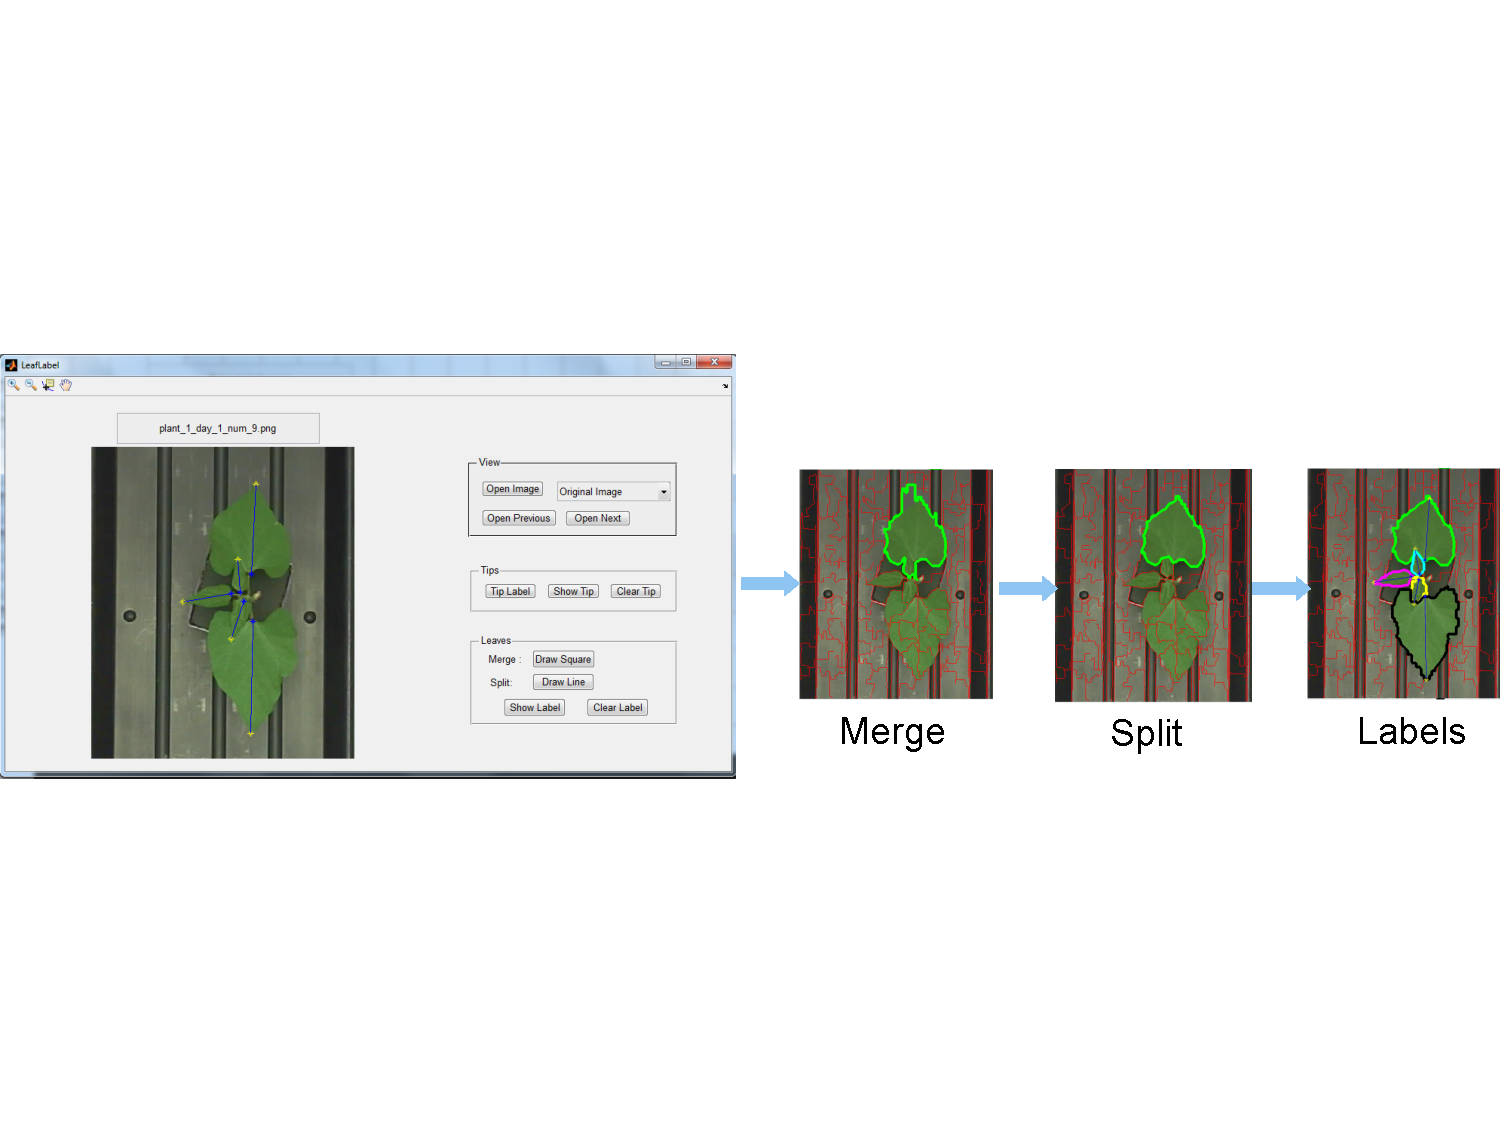
\includegraphics[width=.98\textwidth]{Figures/labeling}\\
\caption{Leaf labeling process, including tip labels and leaf segmentation annotation.}
\label{fig:label}
\end{figure*}

\begin{figure*}
\begin{centering}
\begin{tabular}{@{}c@{} c@{} c@{} c@{} c@{} c@{} c@{} c@{} c@{}}
%\begin{tabular}{lllllllll}
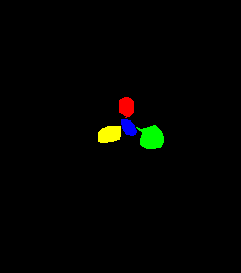
\includegraphics[width=.11\textwidth]{Figures/labelExample/plant_1_day_1_num_13.png}&
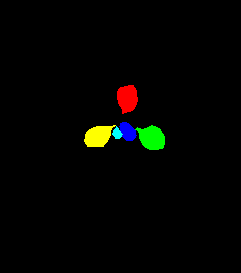
\includegraphics[width=.11\textwidth]{Figures/labelExample/plant_1_day_2_num_13.png}&
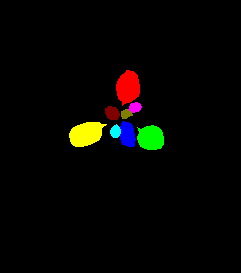
\includegraphics[width=.11\textwidth]{Figures/labelExample/plant_1_day_3_num_13.png}&
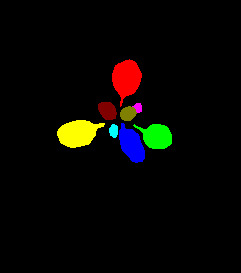
\includegraphics[width=.11\textwidth]{Figures/labelExample/plant_1_day_4_num_13.png}&
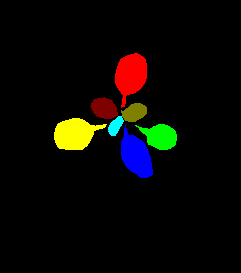
\includegraphics[width=.11\textwidth]{Figures/labelExample/plant_1_day_5_num_13.png}&
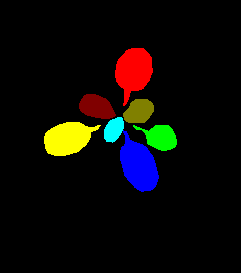
\includegraphics[width=.11\textwidth]{Figures/labelExample/plant_1_day_6_num_13.png}&
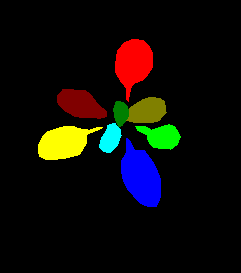
\includegraphics[width=.11\textwidth]{Figures/labelExample/plant_1_day_7_num_13.png}&
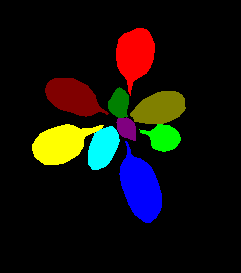
\includegraphics[width=.11\textwidth]{Figures/labelExample/plant_1_day_8_num_13.png}&
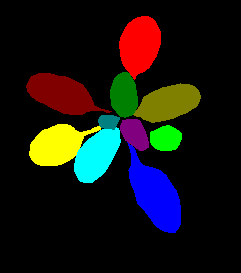
\includegraphics[width=.11\textwidth]{Figures/labelExample/plant_1_day_9_num_13.png}\\
  day 1 & day 2 & day 3 & day 4 & day 5 & day 6 & day 7 & day 8 & day 9 \\
\end{tabular}
\caption{Leaf labeling results of one Arabidopsis plant over nine days with one image per day. Note that the labels of tips are not shown for visualization clarity. }
\label{fig:LabelExample}
\end{centering}
\end{figure*}

The labeling of leaf tips is implemented by clicking pairs of points on the image.
The outer tip is always clicked first before the inner tip.
For visualization, a line connecting each pair of tips will be shown immediately after clicking the inner tip.
Inaccurate labels can be deleted by clicking the right button of the mouse near the labeled point and relabeled by clicking the left button again.

The labeling of the leaf segment is implemented by clicking the boundary of one leaf at each time.
In order to provide more accuracy labeling, we click very dense points ($\sim20$ points on average) on the boundary. 
The labeled leaf boundary is overlaid on the image for better visualization to guide the next action.
Incorrect label can be deleted right after the labeling.
This process continues until all leaf segments have been annotated.
After the labeling of one plant, we visually go through the results and correct inaccurate labels.
One example of the labeling results for one plant is shown in Figure~\ref{fig:LabelExample}, where one color is used to represent each specific leaf.
As we can see during the transition between day $4$ and day $5$, there is one leaf showing up and covering up the leaf underneath, which disappears and will not be annotated later.
In total, we labeled $5142$ leaves.

Note that one alternative approach for labeling leaf segments is to directly label the membership of superpixels instead of drawing a polygon along the boundary.
Our experience is that since a noticeable percentage of extracted superpixels cover pixels of two neighboring leaves, the extra effort of breaking a superpixel into two makes it a less efficient alternative.




\subsection{Name conventions and file types}
We release training and testing sets in two separate folders.
In each folder, there are two subfolders named Arabidopsis and Bean.
The files in each subfolder have the following form:

\begin{itemize}
  \item plant$\_$ID$\_$day$\_$X$\_$hour$\_$YY$\_$rgb.png: the original RGB color images;
  \item plant$\_$ID$\_$day$\_$X$\_$hour$\_$YY$\_$fmp.png: the original fluorescence images;
  \item plant$\_$ID$\_$day$\_$X$\_$hour$\_$YY$\_$ir.png: the original IR images;
  \item plant$\_$ID$\_$day$\_$X$\_$hour$\_$YY$\_$depth.png: the original depth images;
  \item plant$\_$ID$\_$day$\_$X$\_$hour$\_$YY$\_$label.png: the labeled images of fluorescence modality;
  \item plant$\_$ID$\_$day$\_$X$\_$hour$\_$YY$\_$tips.txt: the labeled tip locations;
\end{itemize}
where ID indicates the plant ID number ($1$ to $16$ for Arabidopsis, $1$ to $5$ for bean), X is an integer indicating the date ($1-9$ for Arabidopsis, $1$ to $5$ for bean), and YY represents the image index within a day ($1-16$ for Arabidopsis, $1$ to $14$ for bean).
For each combination of day and hour, we provide four modalities in PNG files ($\_$rgb, $\_$fmp, $\_$ir, $\_$depth).
%\begin{itemize}
%  \item plant$\_$XX$\_$day$\_$X$\_$hour$\_$YY$\_$ID$\_$ZZ$\_$rgb.png: the original RGB color images;
%  \item plant$\_$XX$\_$day$\_$X$\_$hour$\_$YY$\_$ID$\_$ZZ$\_$fmp.png: the original fluorescence images;
%  \item plant$\_$XX$\_$day$\_$X$\_$hour$\_$YY$\_$ID$\_$ZZ$\_$ir.png: the original IR images;
%  \item plant$\_$XX$\_$day$\_$X$\_$hour$\_$YY$\_$ID$\_$ZZ$\_$depth.png: the original depth images;
%  \item plant$\_$XX$\_$day$\_$X$\_$hour$\_$YY$\_$ID$\_$ZZ$\_$label.png: the labeled images of fluorescence modality;
%  \item plant$\_$XX$\_$day$\_$X$\_$hour$\_$YY$\_$ID$\_$ZZ$\_$tips.txt: the labeled tip locations;
%\end{itemize}
%where XX indicates the plant type ("AR" or "BE"), X is an integer indicating the date (e.g., $1-9$ for Arabidopsis), YY represents the image index within a day (e.g., $1-16$ for Arabidopsis), and ZZ is the subject (or plant) ID (e.g., $1-5$ for bean).
%For each combination of day and hour, we provide four modalities in PNG files ($\_$rgb, $\_$fmp, $\_$ir, $\_$depth).
For annotated images, we have two additional files ($\_$label, $\_$tips) saving the annotation results.
Leaf segmentation results are encoded as indexed PNG files, where each leaf is assigned a unique and consistent leaf ID over time.
Leaf ID starts from $1$ and continuously increase till the total number of leaves.
And the background is encoded as $0$.
Tips locations are saved in TXT files where each line has the following format:
\begin{itemize}
  \item leaf ID \quad tip1$\_$x \quad tip1$\_$y \quad tip2$\_$x \quad  tip2$\_$y
\end{itemize}
where leaf ID is an integer number that is consistent with the segmentation label in the PNG file.
tip1$\_$x and tip1$\_$y represent the coordinates of the outer tip point.
tip2$\_$x and tip2$\_$y represent the coordinates of the inner tip point.


In addition to the original images and annotation results, we provide another folder named Matlab with all Matlab functions that will be used for mapping between different image modalities and for the purpose of performance evaluation.
Note that the annotation is provided based on fluorescence images.
In order to evaluate methods developed on other modalities, we provide image mapping functions between every two modalities.
The total storage of our database is around $XX Mb$, which is convenient for downloading via Internet.

\begin{figure*}[t!]
\centering
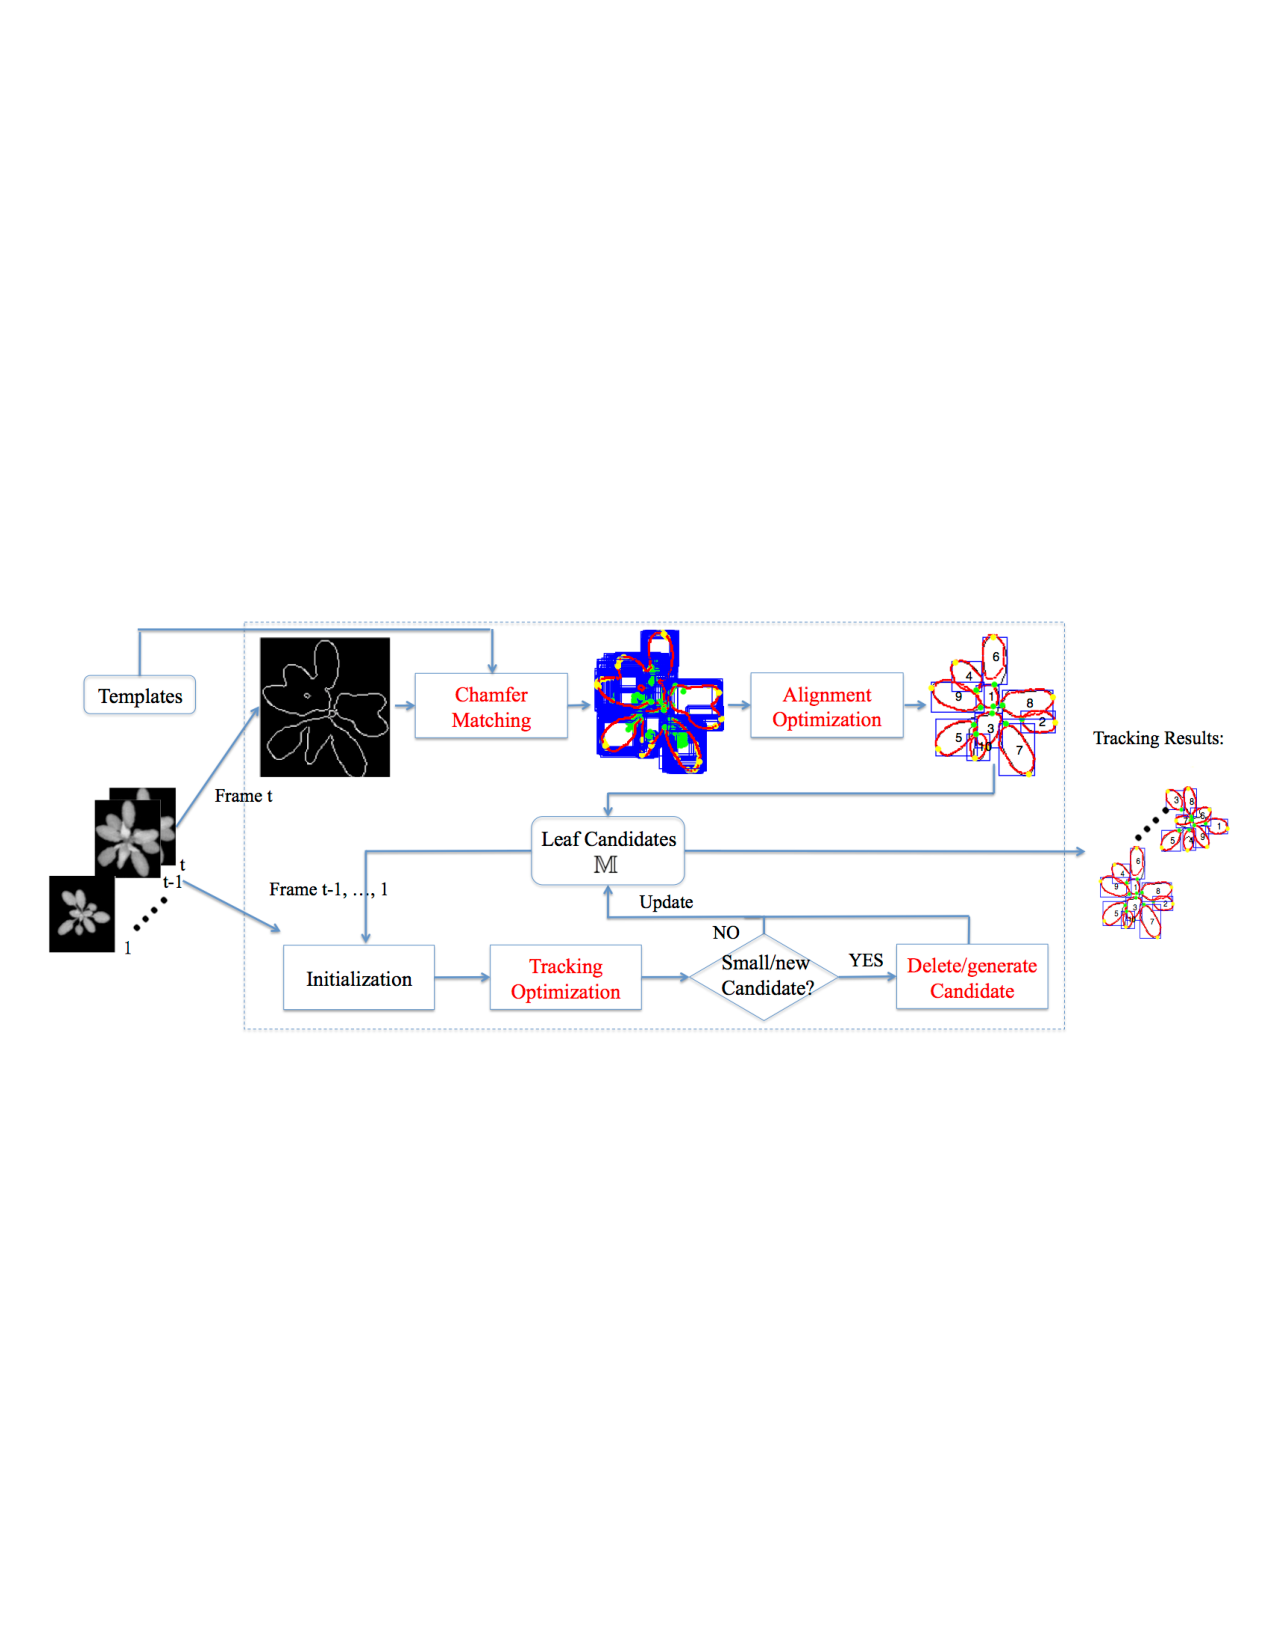
\includegraphics[width=.98\textwidth]{Figures/overview}\\
\caption{Overview of the baseline method.}
\label{fig:methodOverview}
\end{figure*}

\subsection{Experimental Protocols}
As shown in Table~\ref{tab:database}, MSU-PID can be used for applications such as leaf segmentation, leaf alignment, leaf tracking, and leaf counting.
To facilitate future research, we separate the database into the training set and the testing set.
$40\%$ of the data is used for training and $60\%$ for testing.
Specifically, $6$ plants of Arabidopisis and $2$ plants of bean are selected for training.
%We will provide training and testing data in different folders.
For fair comparison, both supervised learning and unsupervised learning methods should evaluate their performances on the training and testing sets separately.
The user may decide to utilize one or multiple modalities of the plant imagery for training and testing respectively.
The availability of multiple modalities allows user to design novel experimental setup.
For example, using RGB and depth modalities for training and RGB for testing can evaluate an algorithm that can handle a missing modality during the testing.
%The evaluation metrics will be discussed in Sec.~\ref{sec:baseline}.



\paragraph{Performance metric}
To evaluate the performance of leaf segmentation, alignment, and tracking, we use four performance metrics, whose Matlab implementations will be provided along with the data.
Three of them are based on the tip-based error, which is defined as the average distance of a pair of estimated leaf tips $\hat{\bm{t}}_{1,2}$ with a pair of labeled leaf tips $ \bm{t}_{1,2}$ normalized by the labeled leaf length:
\begin {equation}
e_{la}(\hat{\bm{t}}_{1,2}, \bm{t}_{1,2}) = \frac{||\hat{\bm{t}}_1-{\bm{t}}_1||_2 + ||\hat{\bm{t}}_2-{\bm{t}}_2||_2}{2 ||\bm{t}_1-\bm{t}_2||_2}.
\label{eqn:tipError}
\end{equation}

We build the frame-to-frame and video-to-video correspondence respectively and generate two sets of tip-based errors.
More details can be find in~\cite{yin2014b}.
We define a threshold $\tau$ to operate on the corresponding tip-based errors.
By varying $\tau$, we compute the first three metrics as follows:
\begin{itemize}
  \item {\it{Unmatched Leaf Rate (ULR)}}, the percentage of unmatched leaves with respect to the total number of labeled leaves.
This can attribute to two sources.
The first is miss detections and false alarms.
The second is matched leaves with tip-based errors larger than $\tau$.
  \item {\it{Landmark Error (LE)}}, the average tip-based errors smaller than $\tau$ of all frame-to-frame correspondent leaves.
  \item {\it{Tracking Consistency (TC)}}, the percentage of video-to-video correspondent leaves whose tip-based errors are smaller than $\tau$.
\end{itemize}

In order to evaluate the leaf segmentation accuracy, we adopt an additional metric~\cite{scharr2014annotated} based on the Dice score of estimated segmentation results and ground truth labels:
\begin{itemize}
  \item {\it{Symmetric Best Dice (SBD)}}, the symmetric best Dice among all labeled leaves.
\end{itemize}
The Matlab function for computing {\it{SBD}} is provided by~\cite{scharr2014annotated}.
The instruction on how to use the evaluation functions are included as comments of the function.


%For leaf annotation, we use the idea of merging and splitting super pixels.
%There are six different numbers of super pixels: $100$, $200$, $300$, $500$, $800$, $1000$.
%The user can specify which level to use depending on how well the super pixels can separate the leaves from the background.
%Because one leaf can be covered by several super pixels and one super pixel can across two leaves or the foreground and background.
%We allow merging and splitting super pixels.
%Merging is implemented by drawing a rectangle on the image.
%Every super pixel overlapping with this rectangle will be merged together.
%Splitting is implemented by drawing a line separating a leaf from the background or from another leaf.
%
%As shown in Fig.~\ref{fig:label}, several super pixels that covers one leaf are first merged together to form a large super pixel.
%Since the top part of the super pixel covers some of the background and the bottom part covers another small leaf, two lines are drawn on this super pixel to split it.
%The leaf boundary is overlaid on the image for better visualization to guide the next action.
%This process continues until all leaves have been annotated.


